\chapter{Realizações}

\section{Revisão bibliográfica}\label{chp:biblio}

Buscando a sanar as dificuldades encontradas relacionadas a calibração da da sobreposição da projeção da realidade aumentada, foram pesquisados referências que esclareçam o fundamento matemático dessa transformação. [Procurar artigo de exemplo].

O vídeo \textit{Augmented Reality: Camera Calibration}, do autor Pavel Rojtberg, detalhou os conceitos da calibração e presentou a abordagem matemática do problema \cite{augmented-calib}. Segundo a conferência, uma projeção em AR pode ser modelada com uma função \(f\) que faz a transformação de um ponto de um espaço 3D (modelo virtual) para um espaço 2D (visualização), definida por: 
\begin{gather*}
    f(P,\,R,\,t,\,C) = p \\
    \text{$p$: ponto (x,y) da projeção; ~$P$: ponto (X,Y,Z) do modelo} \\
    \text{$R$: parâmetro de rotação; ~$t$: parâmetro de translação} \\
    \text{$C$: parâmetro de distorção da câmera} 
  \end{gather*}
Os parâmetros R e t são matrizes descrevem a rotação e a posição da câmera que, em condições normais, são constantes e chamados de parâmetros extrínsecos da câmera. O parâmetro C é uma matriz que modela as deformações da construção da lente da câmera, particular para cada dispositivo de captura de imagem. As deformações variam sua intensidade e modo de 

\begin{figure}[H]
    \centering
    \begin{subfigure}{.45\textwidth}
        \centering
        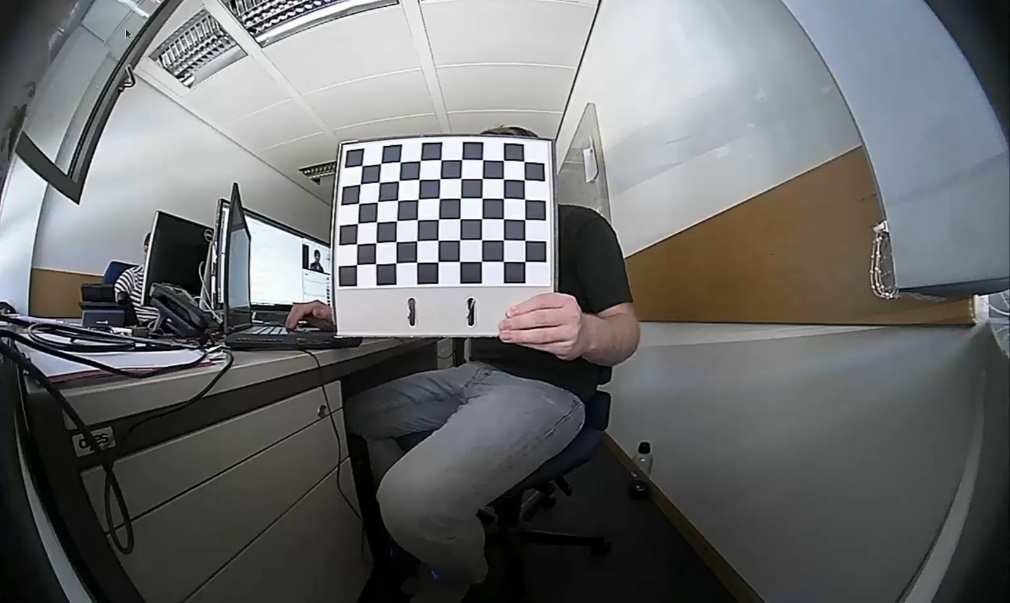
\includegraphics[width=.95\linewidth]{figuras/CaptureReal.png}
        \caption{Imagem real da câmera.}
        \label{fig:cap-real}
    \end{subfigure}
    \begin{subfigure}{.45\textwidth}
        \centering
        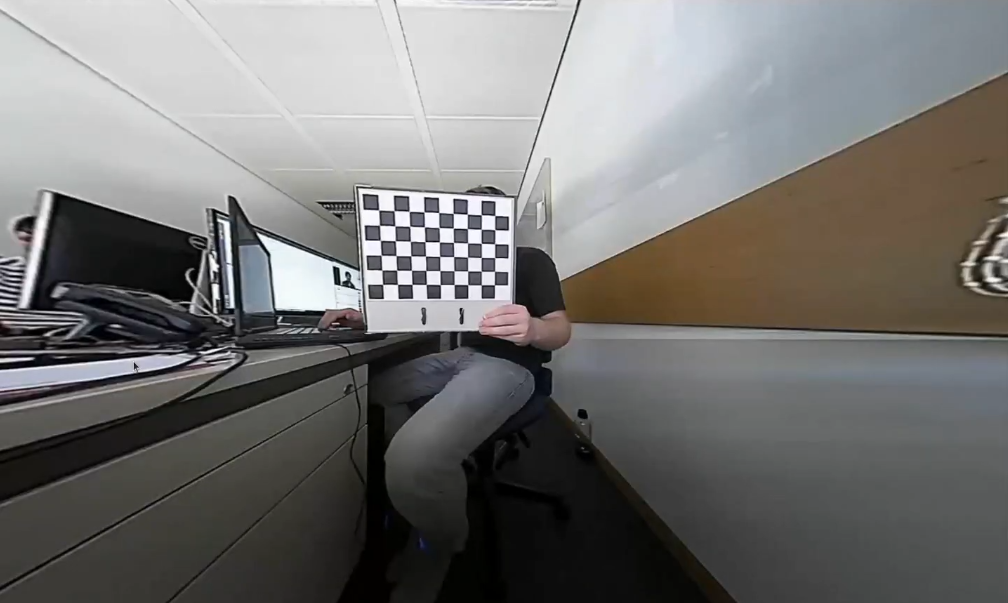
\includegraphics[width=.95\linewidth]{figuras/CaptureFixed.png}
        \caption{Imagem corrigida.}
        \label{fig:cap-fix}
    \end{subfigure}
    \caption{Comparação entre imagem real da captura e imagem corrigida. Fonte: \cite{augmented-calib}.}
    \label{fig:capture-comp}
\end{figure}

\begin{figure}[H]
    \centering
    \begin{subfigure}{.45\textwidth}
        \centering
        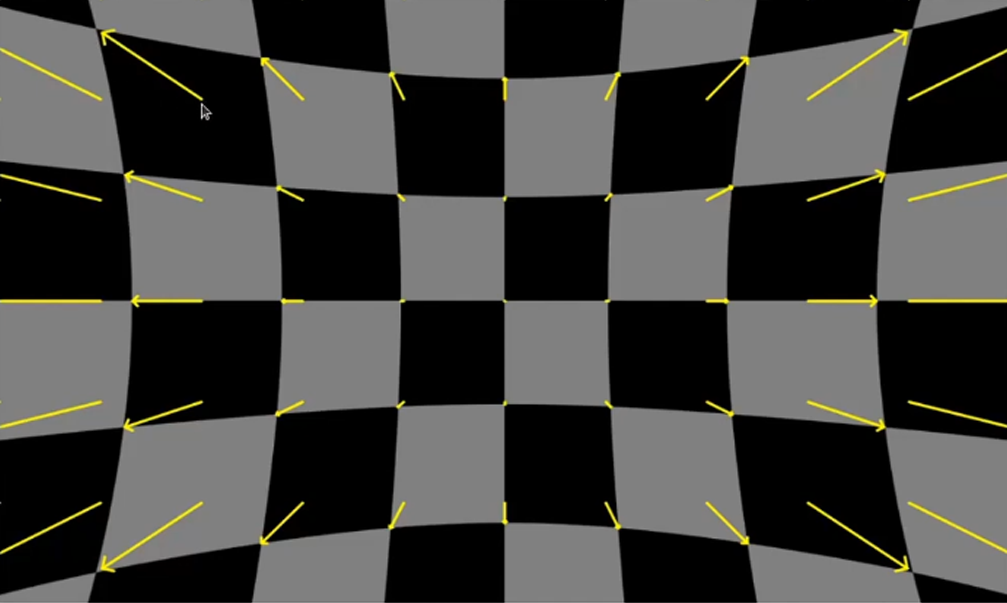
\includegraphics[width=.95\linewidth]{figuras/DistortionRadial.png}
        \caption{Distorção radial.}
        \label{fig:radial}
    \end{subfigure}
    \begin{subfigure}{.45\textwidth}
        \centering
        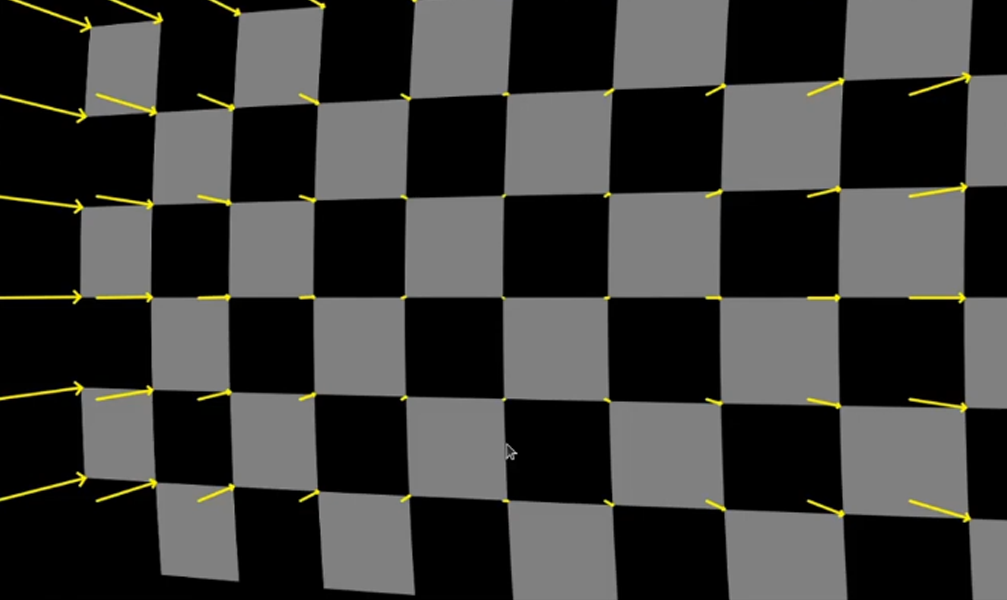
\includegraphics[width=.95\linewidth]{figuras/DistortionTang.png}
        \caption{Distorção tangencial.}
        \label{fig:tangencial}
    \end{subfigure}
    \caption{Exemplo dos tipos de distorção das câmeras. Fonte: \cite{augmented-calib}.}
    \label{fig:distort-comp}
\end{figure}

A deformação pode ser separada em duas componentes: radial e tangencial (Figura \ref{fig:distort-comp}). Em \textit{webcams} convencionais, podemos encontrar com frequência ambas as componentes de distorção, porém em câmeras de alta qualidade de fabricação, é comum encontrar somente deformação radial, por conta do formato das lentes ser circular e muitas utilizam essa estrutura para ampliar seu ângulo de visão, como acontece com as lentes \textit{fisheye} (Figura \ref{fig:cap-real}). 

\begin{figure}[H]
    \centering
    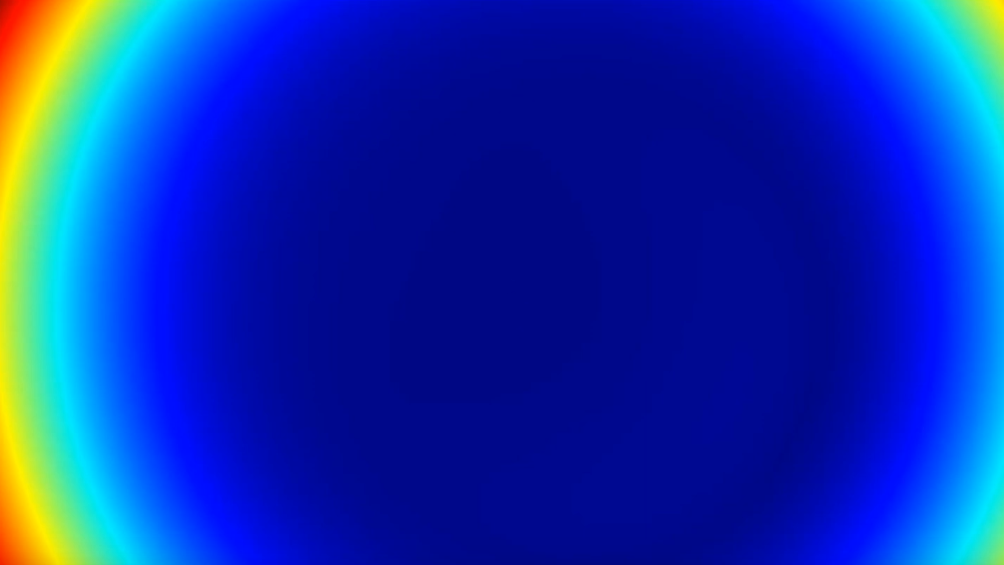
\includegraphics[width=.5\linewidth]{figuras/Distortion Color.png}
    \caption{Diagrama da distorção de captura de uma câmera, contendo componente radial e tangencial. Regiões azuis são menos afetadas e regiões vermelhas são mais afetadas pela distorção. Fonte: \cite{augmented-calib}.}
    \label{fig:distort-diagram}
\end{figure}

\section{VCranium}\label{chp:vcranium} 

Durante o primeiro período de um ano da pesquisa, foi possível definir uma arquitetura adequada para a aplicação à AR em neurocirurgias e um nome fantasia: \textit{VCranium}. Em sumo, o sistema foi dividido em computador e óculos: O computador estima a posição da projeção e os óculos exibem as imagens nos olhos do usuário. Esse sistema foi inspirado no artigo de Maruyama, que utilizou um \textit{software} de visualização médica em um computador, que fazia o envio dos dados para os óculos \textit{AR} utilizando o \textit{Unity} \cite{Maruyama2018}.

\begin{figure}[ht]
    \centering
    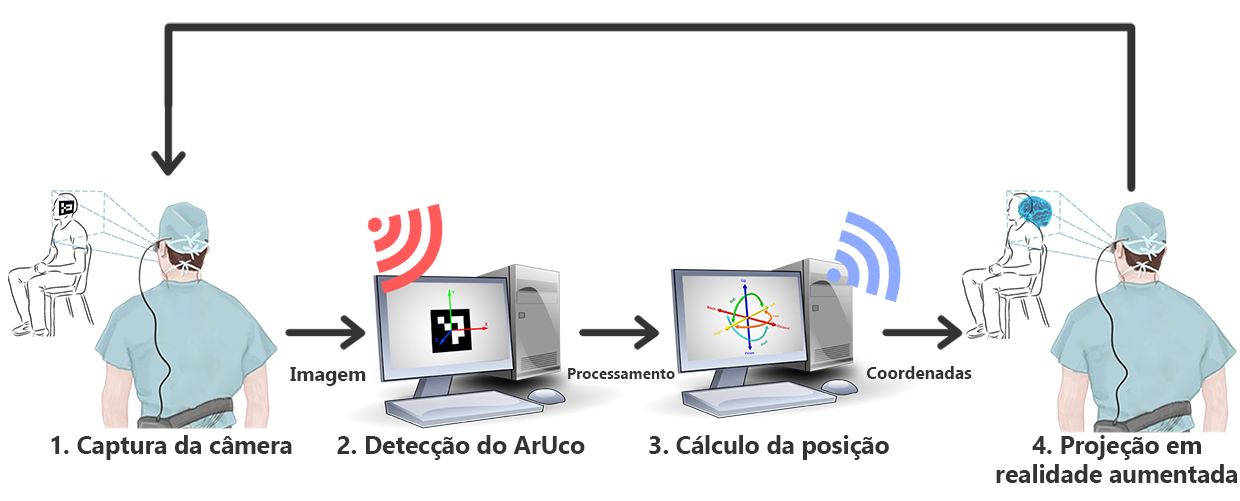
\includegraphics[width=.9\linewidth]{figuras/System schematic.png}
    \caption{A figura representa o funcionamento do sistema. (1) Captura a imagem do paciente e envio para o computador. (2) Faz uma varredura na imagem e identifica o marcador ArUco. (3) Calcula a posição do marcador e envia as coordenadas para os óculos. (4) Recebe as informações e exibe a projeção para o usuário e então retorna para o passo 1. Fonte: Autor.}
    \label{fig:arc}
\end{figure}

\section{Calibração}

A \textit{OpenCV Library} implementou um método que permite medir a deformação de cada câmera com o fim de gerar os parâmetros da calibração. Esse processo é feito utilizando um marcador especial apelidado pela documentação por \textit{''chess board''}, que serve de ferramenta para o programa encontrar a distância de cada vértice de quadrado entre si e, dessa maneira, calcular os coeficientes de distorção \cite{opencv-calib}. Por fim, podemos visualizar o processo na Figura \ref{fig:chessb}, a documentação sugere que ao menos 10 amostras sejam feitas e, em cada imagem, os pontos são encontrados pelo programa e utilizados para o cálculo dos parâmetros.

\begin{figure}[ht]
    \centering
    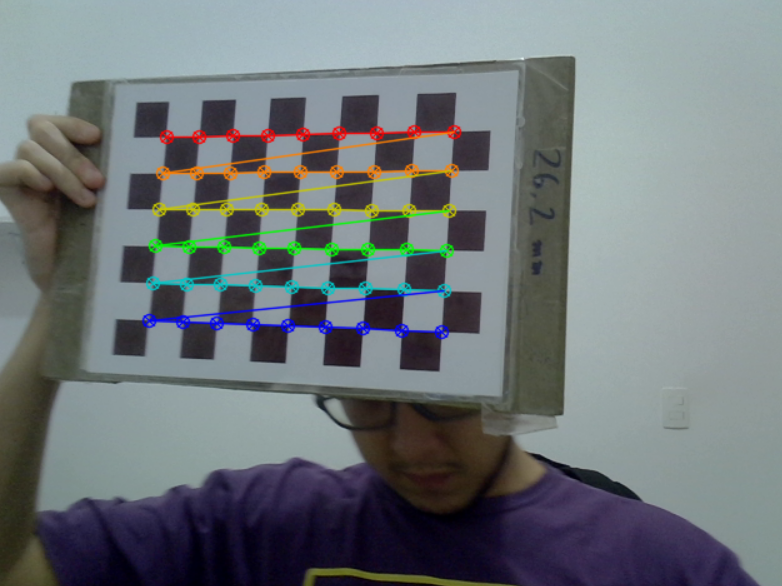
\includegraphics[width=.4\linewidth]{figuras/chessboard.png}
    \caption{Processo de calibração da câmera. Fonte: Autor.}
    \label{fig:chessb}
\end{figure}

Após esse último processo, utilizamos os parâmetros encontrados para realizar a estimação da posição do marcador \textit{ArUco}, como já foi feito na entrega anterior Figura \ref{fig:error-calib}. Como foi descrito também no último relatório, não foi possível adquirir um resultado satisfatório sobre a calibração da projeção AR. 

\begin{figure}[ht]
    \centering
    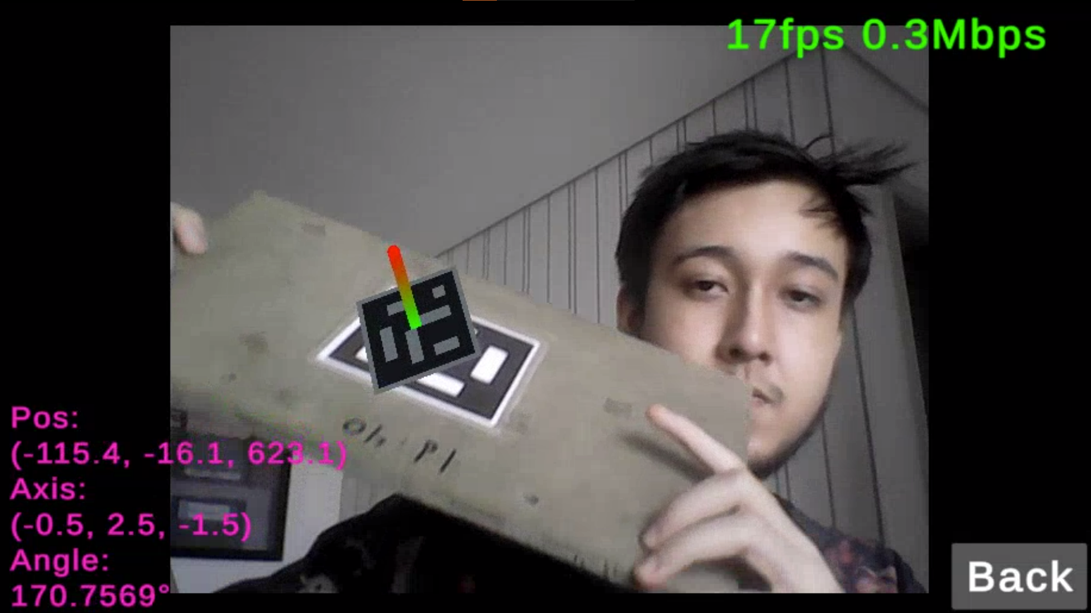
\includegraphics[width=.4\linewidth]{figuras/vcranium_calibration.png}
    \caption{Projeção AR sem calibração, adquirida na entrega anterior. Fonte: Autor.}
    \label{fig:error-calib}
\end{figure}

Compreendendo a abordagem do assunto apresentado por Pavel e a divisão entre parâmetros extrínsecos e intrínsecos da projeção, foi possível representar o problema enfrentado pelo projeto na Figura \ref{fig:calib-proj-comp}.

\begin{figure}[H]
    \centering
    \begin{subfigure}{.4\textwidth}
        \centering
        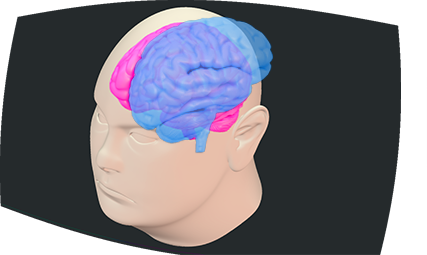
\includegraphics[width=.65\textwidth]{figuras/CalibNot2.png}
        \caption{Sem calibração.}
        \label{fig:calib-proj-without}
    \end{subfigure}
    \begin{subfigure}{.4\textwidth}
        \centering
        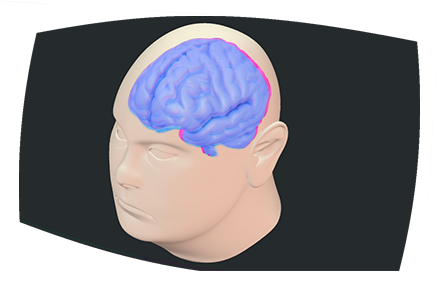
\includegraphics[width=.65\textwidth]{figuras/CalibExtr.png}
        \caption{Calibração somente extrínseca.}
        \label{fig:calib-proj-extr}
    \end{subfigure}
    \begin{subfigure}{.4\textwidth}
        \centering
        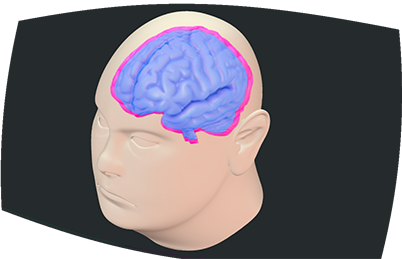
\includegraphics[width=.65\textwidth]{figuras/CalibIntr.png}
        \caption{Calibração somente intrínseca.}
        \label{fig:calib-proj-intr}
    \end{subfigure}
    \begin{subfigure}{.4\textwidth}
        \centering
        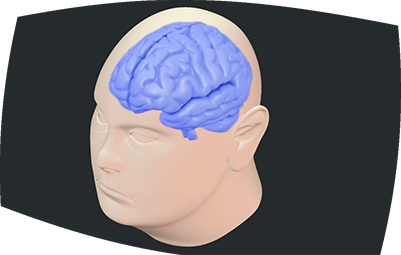
\includegraphics[width=.65\textwidth]{figuras/Calib.png}
        \caption{Calibração extrínseca e intrínseca.}
        \label{fig:calib-proj}
    \end{subfigure}
    \caption{Comparação da combinação de cada componente de calibração. Fonte: Autor.}
    \label{fig:calib-proj-comp}
\end{figure}

\section{Implementação}\label{chp:impl}

A figura \ref{fig:calib-proj-comp} facilita a explicação dos problemas enfrentados pela calibração AR. O primeiro exemplo da Figura \ref{fig:calib-proj-without}, representa o problema encontrado pela última entrega (Figura \ref{fig:error-calib}) que consiste na total inconsistência de orientação do modelo em relação à referência. Para solucionar isso, foi implementado ajustes no código em \textit{C\#} da plataforma \textit{Unity} para realizar um ajuste de posição e rotação manual. Podemos verificar isso com a Figura \ref{fig:extr-comp}.

\begin{figure}[H]
    \centering
    \begin{subfigure}{.45\textwidth}
        \centering
        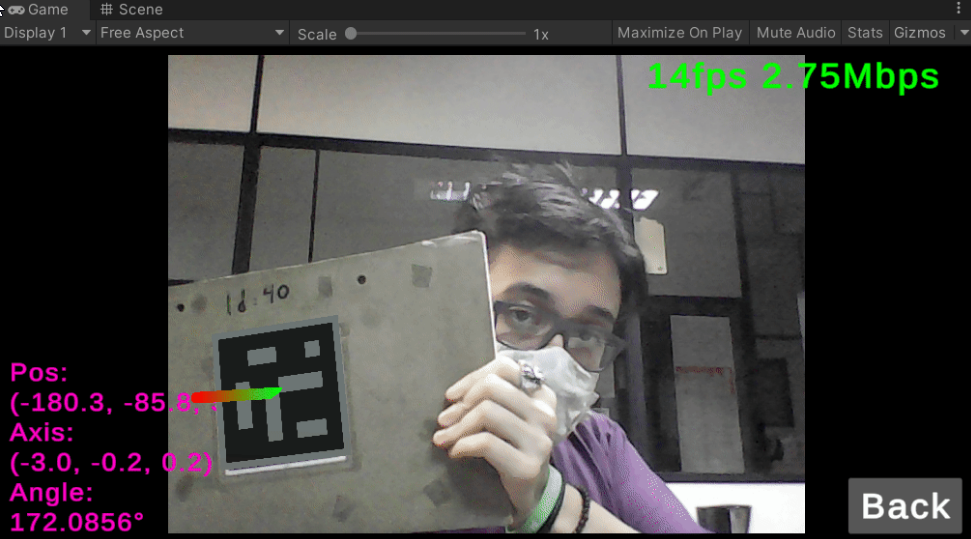
\includegraphics[width=.95\linewidth]{figuras/vcranium-extr1.png}
        \caption{Exemplo de projeção calibrada.}
        \label{fig:extr1}
    \end{subfigure}
    \begin{subfigure}{.45\textwidth}
        \centering
        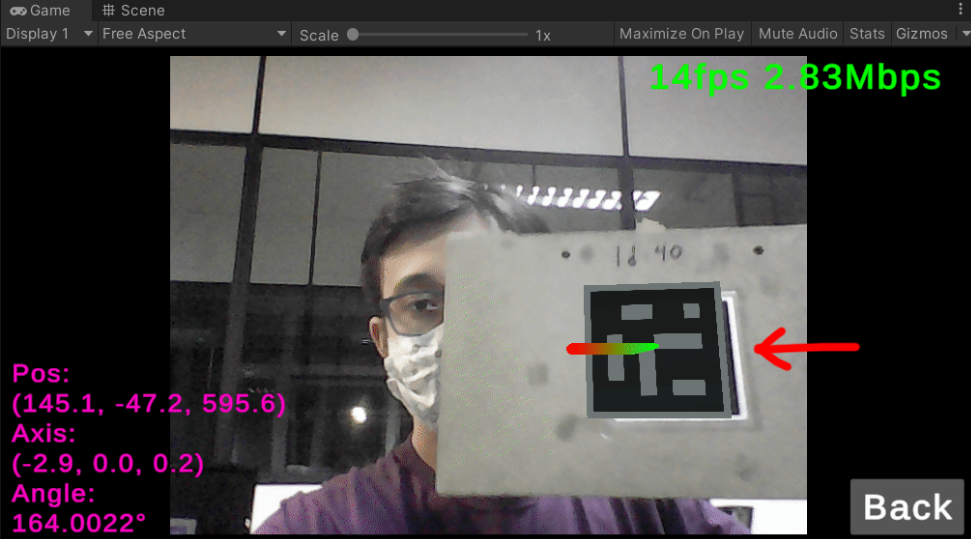
\includegraphics[width=.95\linewidth]{figuras/vcranium-extr2.png}
        \caption{Modificação do erro da projeção.}
        \label{fig:extr2}
    \end{subfigure}
    \caption{Visualização da projeção após a calibração extrínseca por \textit{Unity}. Fonte: Autor.}
    \label{fig:extr-comp}
\end{figure}

Foi possível perceber na prática que o ajuste de rotação e posição da projeção é o mesmo que uma calibração extrínseca, por isso, observando a Figura \ref{fig:extr1}, a projeção sobrepõe bem o marcador, porém, na mesma configuração, o mesmo não ocorre em outra região da tela. A Figura \ref{fig:extr2} mostra que erro da projeção se altera conforme mudamos a posição do marcador no mundo real, mostrando que não há solução constante de rotação e posição que realize uma sobreposição consistente em todas as partes da tela.

Esse fenômeno é causado pelas diferentes deformações que a imagem da câmera possui, visto também no diagrama da Figura \ref{fig:distort-diagram}. Nesse exemplo, a projeção pode ser muito boa nas regiões azuis da imagem, porém, obtemos erros grandes nas regiões vermelhas. A ilustração criada na Figura \ref{fig:calib-proj-comp} consiste em uma imagem muito deformada, i.e, a imagem toda possui um grau de deformação radial e tangencial. Isso implica na impossibilidade da sobreposição ocorrer ao utilizar a calibração puramente extrínseca, como é observado em \ref{fig:calib-proj-extr}, observamos que a projeção terá um erro variável em sua extensão.